\section{Introduction}\label{intro}\sloppy


Data cleaning is widely recognized as a major challenge in almost all forms of data analytics~\cite{nytimes}, and analysts may spend upwards of 80\% of the analysis effort to clean and prep the data.  A common form of data errors are those where attribute values are incorrect---these errors can vary from missing data, incorrect or biased values, misspellings, the concatenation of multiple attributes due to extraction errors, and more.  These errors must be fixed before being used by downstream applications such as SQL queries, visualizations, or machine learning models.    

\begin{figure}[t]
  \centering
 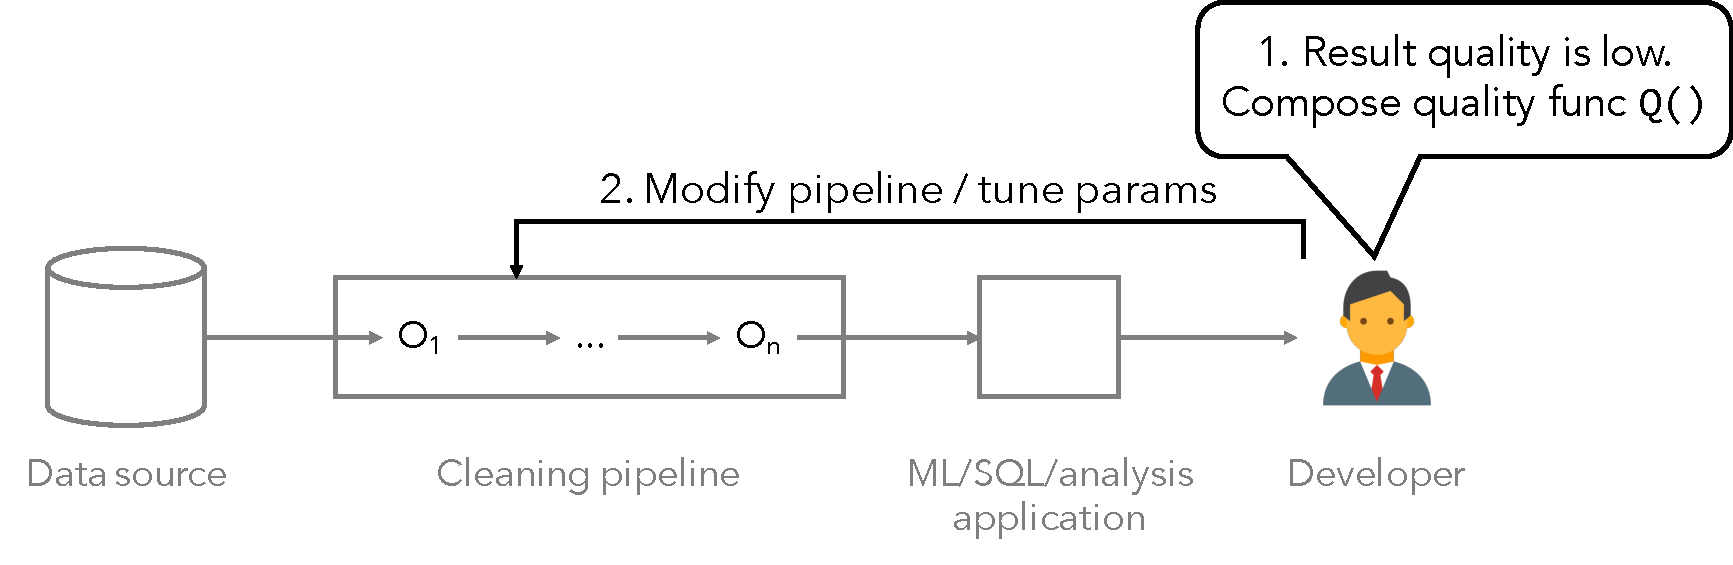
\includegraphics[width=\columnwidth]{figures/user-pipeline}
 \caption{\small Typical data cleaning pipeline.  The user finds that analysis results (of SQL query, ML model, web application, etc) are suspicious and iteratively (1) composes a quality function to characterize the suspicious quality issues, and (2) modifies the data cleaning pipeline to address the errors.  The bottleneck is the human-in-the-loop.  \label{fig:teaser}}
\end{figure}



Data cleaning is challenging because there is rarely a well-defined ground-truth. Instead, developers must both 1) characterize the data quality issues that affect their application, and 2) compose data cleaning programs to fix those issues.  However, this is challenging for three reasons.  First, developers often do not know the exact description nor the extent of the quality issues of their data up-front.  Instead, the issues are revealed by examining analysis output and throughout the cleaning process~\cite{krishnan2016hilda}.    We call this a quality function, modeled as a function $Q(\mathcal{D}) \in [0, 1]$ over the dataset $\mathcal{D}$ that returns $1$ if there are no discernable quality issuues, lower values correspond to a dirtier table.

Second, developers must translate these quality characteristics into a data cleaning program that fixes these errors.  This is done by choosing and combining data cleaning systems and operations and checking their effects on the data quality and downstream application.  For instance, specialized systems such as HoloClean~\cite{}, XXX~\cite{}, and others~\cite{} are designed to detect specific types of data errors, and generate fixes for them.  


However, even for a simple logical cleaning operator, such as outlier value imputation, there is a large space of physical cleaning options.  Which  outliers could utilize a fixed threshold, an unsupervised statistical model, a problem-specific model (e.g., of EEG signals~\cite{}), a based on constraints.  Each operation further burdens the developer with numerous choices to set its parameters---what threshold?  How many clusters? What model features?   Once the outliers have been detected, there is a similar buffet of options to actually replace the outlier value.     Unfortunately, data cleaning is challenging because even a single data set can have many different types of errors (e.g., outliers, constraint violations, duplicates, mis-spellings, incorrect orderings).

The third, more subtle issue, is that it is easy to confound the quality function and the cleaning program because they are seemingly related.  

It is a human in the loop problem.


Specialized operators are tailored to specific error types and fix operators.

Pipelines are flexible, but requrie the developer to reason about a large search space.

Ideally, user primarily focuses on quantifying the error types, and the allows the system to generate cleaning programs, refining the search space as desired.

One promising approach is hyperparameter search.

It doesn't work.  Teaser example

Our paper 1) encodes cleaning objectives as a quality function, and provides tools for users to compose quality functions easily, 2) models cleaning as a sequential learning problem, 3) uses machine learning to dynamically prune the search space during the search process.  



Ultimately, data cleaning is a human-in-the-loop process driven by the user's domain expertise.  Thus, the input and output interfaces should be flexible and optimized for the user.   Users should be able to easily specify, and rapidly refine, potentially arbitrary {\it data-quality measures}.  It should also be easy to pick data transformation operators from a pre-existing library, or wrap specialized data cleaning libraries as user-defined operators.  To ensure that the system output is easy to understand, the system should generate simple programs composed of the user-specific transformation operators, rather than directly fixing the database contents.

A naive approach is to layer a black-box hyper-parameter tuning algorithm on an existing data cleaning framework.  The selection of operators, how they are combined, and how their parameters are set, can be modeled as a separate hyperparemeter that an optimization algorithm such as X, Y, or Z will explore.  The user's task is to specify and tune the optimization objective to lead the search towards an acceptable solution.   \ewu{THere's a gap here that I'm missing}

However this approach ignores important aspects of data cleaning problems that enable more efficient and flexible approaches.  First, data cleaning programs are often a sequence of transformations applied one after the other, thus the entire space of hyperparameters does not need to be learned jointly.  Second, a given transformation may be applied multiple times, whereas a black-box hyperparameter search algorithm would need to know up front the maximum set of trnsaforamiotns and the parameters. Third, the transformations are not commutative, and prior transformations can affect subsequent transformations.  This meoans that local decisions need to account for how they may affect later transformations.  


%Automated data cleaning takes as input a {\it specification} that characterizes the errors in the dataset, as well as a set of allowable {\it data transformations} (e.g., \texttt{set(rowi, attrj, val)}), and automatically applies these transformations to fix the errors.  

% Data  cleaning is composed of pipelines.  in some cases, the pipelines are largely fixed, and developers adjust the parameters of operators in the pipeline, or the pipeline itself, in response to changes in the input data.  In other cases, the core set of parameterized operators are know apriori, but the specific parameterization and pipeline of operators that should be run to achieve a desired data cleaning goal is not clear up front. The latter can happen at a regular basis as new data cleaning scenarios arise (say, due to new customers), a new data source is added to an analysis, or when a data source changes substantially.  In these cases, developers must construct the pipeline and parameterization in order to achieve an often ill-defined cleaning goal.





A starting point is the recent work on systems for \emph{hyperparameter tuning} for machine learning~\cite{li2017hyperband, sparks2017keystoneml, baylor2017tfx, golovin2017google, liaw2018tune}.
These systems are alternatively described as ``black box'' search algorithms as they make few assumptions about the underlying structure of the parameter space---simply put, generality at the cost of runtime.
In machine learning, the objective of the search process is clear: the prediction error on a validation set gives an estimate of accuracy. 
In data cleaning, there is a chicken-and-egg problem, where accuracy is defined in terms of recovering the true values of cells in a database, but knowing the true values in advance would defeat the purpose of cleaning.
In practice, we often use a proxy for accuracy such as the satisfaction of integrity constraints, how well it fits a statistical model, or accuracy on gold standard data.
Given one of these proxy accuracy metrics, is black-box hyperparameter tuning sufficient for applications in data cleaning optimization?

We implement this search framework in a system called \sys.
\sys is provided with a library of data cleaning components and specification of their free parameters. 
We assume that each component specifies its repairs in terms of cell-replacement, the same model as in recent systems like Holoclean~\cite{rekatsinas2017holoclean}.
A parameter generator thread supplies assignments to each of the data cleaning methods in the library and yields candidate repairs as they are generated to a set.
A greedy tree-search algorithm runs in parallel by sequencing candidate repairs and computing the resulting accuracy measure.
\sys can also execute in a divide-and-conquer fashion by generating candidate parameters on different partitions of data.
It also provides utilities for leveraging information across partitions, by learns a prediction model to estimate the expected improvement of different transformation operators (e.g., some library components might be irrelevant).  

\noindent Our contributions include:
\begin{itemize}[leftmargin=*, topsep=0mm, itemsep=0mm]
  \item Rethinking parameter optimization in data cleaning and data transformation with a novel candidate-search framework called \sys. \sys includes an API for specifying data cleaning operations as well as accuracy metrics.
  \item A suite of pragmatic optimizations, such as fast pruning using predictive models, multi-node parallelization, and data sharing to reduce network communication bottlenecks, that reduce the runtime by \ewu{XXX$\times$}.
  \item A systematic study of the benefits and limitations of \sys in terms of data cleaning accuracy (precision, recall), and the runtime.  We show that \sys can solve incremental refinements of the data quality measure $yyy\times$ faster than from scratch, and that \ewu{SOME OTHER FINDING}
\end{itemize}


